\section{Einleitung} 

\begin{frame}\frametitle{Einleitung} 
	\begin{itemize}
		\item Interhyp AG ist Vermittler für private Baufinanzierungen
		\item Primäres Ziel des Marketing ist die Kundenakquise
		\item Etwa $80 \%$ aller Kundenanträge werden online abgeschickt
		\item Online-Marketing verfügt über verschiedene Kanäle
		\item Refined Labs GmbH ist verantwortlich für das Online-Tracking der Werbekampagnen der Interhyp AG
	\end{itemize}
\end{frame}

\begin{frame}\frametitle{Entstehung eines Funnels (Quelle: Interhyp AG)}
	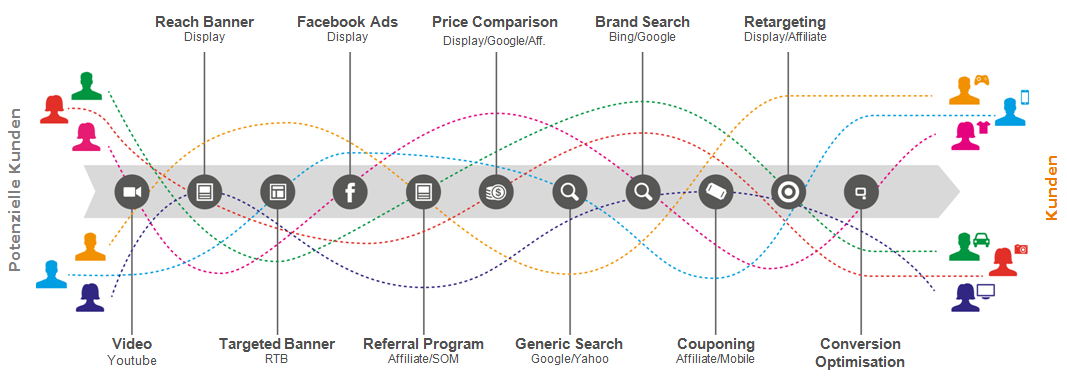
\includegraphics[scale=0.38]{customerJourney.png}\\
	\centering Unterschiede zwischen konvertierten und nicht-konvertierten Funnels?
\end{frame}